%!TEX program = xelatex
%Template created by: Maciej Byczko
\documentclass[a4paper,12pt]{extarticle}  %typ dokumentu

% \usepackage[utf8]{inputenc} %rodzaj czcionki w dokumencie
\usepackage{geometry} %poprawienie marginesów
\usepackage{polski} %polskie znaki
\usepackage{multirow} %tabela
\usepackage{graphicx} %tabela
\usepackage{float} %poprawienie pozycji
\usepackage{fancyhdr} % header i footer
\usepackage{karnaugh-map} % rysowanie siatek karnaugh
\usepackage{hyperref} %tworzenie odnośników, \url{<url>}, \href{<file path, link>}{<text with link>} \pageref{}
\usepackage{amsmath} % Matma
\usepackage{boldline}%edytowanie grubości krawędzi w tabelach \hlineB{} \clineB{}{}
\usepackage{array}%grubsze kolumny w tabeli
\usepackage{bigstrut}
\usepackage{caption}
\usepackage{listings} %pisanie kodu w ładny sposób, begin{listings}[language=<język>]...end{listings} tak samo jak nazwa paczki
\usepackage{subcaption}

%Ustawienie paczki hyperref
\hypersetup{
     colorlinks,
     citecolor=black,
     filecolor=black,
     linkcolor=black,
     urlcolor=black
}

\definecolor{backcolour}{rgb}{0.95,0.95,0.92}
\definecolor{AO}{rgb}{0,0.5,0}
\definecolor{ZeroBlue}{rgb}{0,0.28,0.73}
\definecolor{DarkRed}{rgb}{0.85,0.16,0.16}

\lstset{
breaklines=true,
language=vhdl,
numbers=left,
tabsize=2,
numberstyle=\tiny,
backgroundcolor=\color{backcolour},
breakatwhitespace=false,
showspaces=false,                
showstringspaces=false,
showtabs=false,
commentstyle=\color{gray},
keywordstyle=\color{ZeroBlue},
% keywordstyle={[2]\color{DarkRed}},
% keywordstyle={[3]\color{ZeroBlue}},
}
\graphicspath{{pictures/}}
\geometry{margin=0.7in}
\pagestyle{fancy}

\cfoot{Strona \thepage}
\rhead{Strona \thepage}
\lhead{\typdoc}
\newcolumntype{?}{!{\vrule width 1.5pt}}

\title{\tytul}
\author{\tworcy}
\date{\data}

%-----------------------PRZYDATNE LINKI----------------------------------
%link do tworzenia tabeli https://tablesgenerator.com
%symbole matematyczne: https://oeis.org/wiki/List_of_LaTeX_mathematical_symbols
%narzędzia matematyczne: https://en.wikibooks.org/wiki/LaTeX/Mathematics
%krótkie podpowiedzi http://www.mif.pg.gda.pl/homepages/sylas/students/wdi/doc/latex-sciaga.html
%symbole do schematów: http://texdoc.net/texmf-dist/doc/latex/circuitikz/circuitikzmanual.pdf
%----------------------------------------------------------------------

%-----------------------SEKCJA DANYCH----------------------------------
\def\tytul{Układy wielobitowych wejść i wyjść} %<<< tytuł ćwiczenia
\def\nrcw{4} %<<< numer ćwiczenia
\def\data{8 Listopada 2021r.} %<< data wykonania
\def\prowadzacy{dr inż. Jacek Mazurkiewicz} %<<<prowadzący
\def\nrgrupy{B} %<<<numer grupy
\def\tworcy{Maciej Byczko\\Bartosz Matysiak} %<<< autorzy
\def\zajinfo{PN 10:50 TP} %<<< informacje dotyczące zajęć
\def\typdoc{Sprawozdanie} %<<< typ dokumentu tj Sprawozdanie, zadania itp. {Matematyka dyskretna/Sprawozdanie z Miernictwa}
\begin{document}
\setlength{\headheight}{15pt}

\newcommand{\ov}[1]{\overline{#1} \ }

%-------------------------------------TABELA-DANYCH--------------------------------------------------
\begin{table}[H]
	\centering
	\resizebox{\textwidth}{!}{
		\begin{tabular}{|c|c|c|}\hline
			\begin{tabular}[c]{@{}c@{}}                     \tworcy     \end{tabular} &
			\begin{tabular}[c]{@{}c@{}}Prowadzący:\\        \prowadzacy \end{tabular} &
			\begin{tabular}[c]{@{}c@{}}Numer ćwiczenia\\    \nrcw       \end{tabular}          \\ \hline
			\begin{tabular}[c]{@{}c@{}}                     \zajinfo    \end{tabular} &
			\begin{tabular}[c]{@{}c@{}}Temat ćwiczenia:\\   \tytul      \end{tabular} & Ocena: \\ \hline
			\begin{tabular}[c]{@{}c@{}}Grupa:\\          \nrgrupy    \end{tabular}    &
			\begin{tabular}[c]{@{}c@{}}Data wykonania:\\    \data       \end{tabular} &        \\ \hline
		\end{tabular}}
\end{table}
%----------------------------------------------------------------------------------------------------
\tableofcontents
\cleardoublepage
\section{Zadanie 1}
\subsection{Polecenie}
Detektor 2-znakowej sekwencji słów 8-bitowych: wejścia 2 znaków 8-bitowych, 
1 wyjście 1-bitowe – sekwencja rozpoznana / sekwencja błędna. Źródło danych: 
początkowo "guziki" przystawki, potem klawiatura PC via terminal. 
\subsection{Rozwiązanie}
Do rozwiązania problemu wymagane jest od nas podłączenie dwóch komparatorów 8-bitowych (COMP8), 
które po pobraniu wartości od użytkownika kolejno po sobie sprawdzają wprowadzone słowa.
W zależności od wymagania można wprowadzić także obowiązkowe wprowadzanie wartości w odpowiedniej kolejności.
\subsubsection{Schemat stanów}
% \subsubsection{Tabela prawdy}
% \subsubsection{Siatki Karnaugh}
\subsubsection{Schematy układu} %myślę, że tu damy oba schematy: bez i z obsługą klawiatury, na razie daję ten pierwszy
Schemat dla wersji z przyciskami jako inputem:
\begin{figure}[H]
	\centering
	\resizebox*{\textwidth}{!}{
		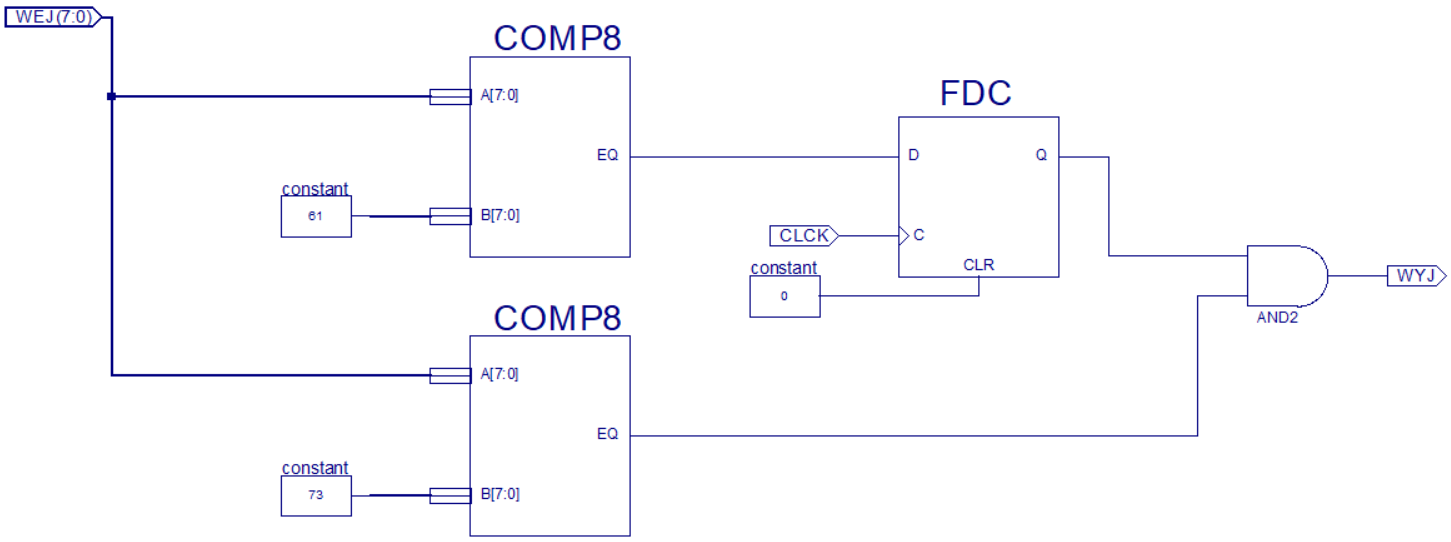
\includegraphics{zadanie1/zad1_scheme_button_input.png}
	}
\end{figure}
Schemat wersji wykorzystującej klawiaturę jako wejście:
% na morzu hula hulami, wieje wieje wiatr
\subsubsection{Kod VHDL}
\lstinputlisting{zadanie1/testbench.vhd}
\subsubsection{Symulacja}
\begin{figure}[H]
	\centering
	\resizebox*{\textwidth}{!}{
		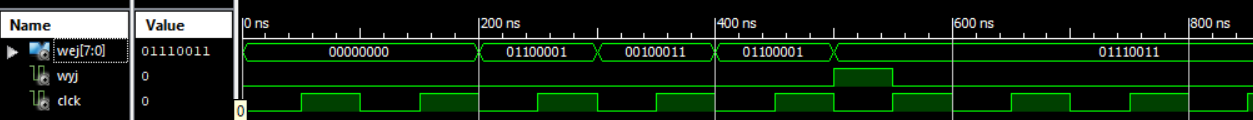
\includegraphics{zadanie1/zad1_simulation.png}
	}
\end{figure}
\subsection{Fizyczna implementacja}
\subsubsection{Kod UCF}
Kod dla wersji z przyciskami jako inputem:
\lstinputlisting{zadanie1/ZL-9572.ucf}
Schemat wersji wykorzystującej klawiaturę jako wejście:
% na morzu hula hulami, wieje wieje wiatr
\section{Zadanie 2}
\subsection{Polecenie}
Układ arytmetyczny pracujący na dwóch argumentach 4-bitowych wyrażonych w kodzie Aikena
i generujący stosowny wynik w tymże kodzie. 
\subsection{Rozwiązanie}
%\subsubsection{Schemat stanów} % pozwolę sobie zauważyć, że stanów, w układach kombinacyjnych, takim jak ten, nie ma
%Dałbym bardziej cos w rodzaju notki wstępnej, np.
\subsection{Uwagi wstępne}
% i tu opis ogólnej struktury układu

\subsubsection{Tabele prawdy} %liczba mnoga; tabele dla każdego podukładu
\subsubsection{Siatki Karnaugh}
\subsubsection{Schemat układu}
\begin{figure}[H]
	\centering
	\resizebox*{\textwidth}{!}{
		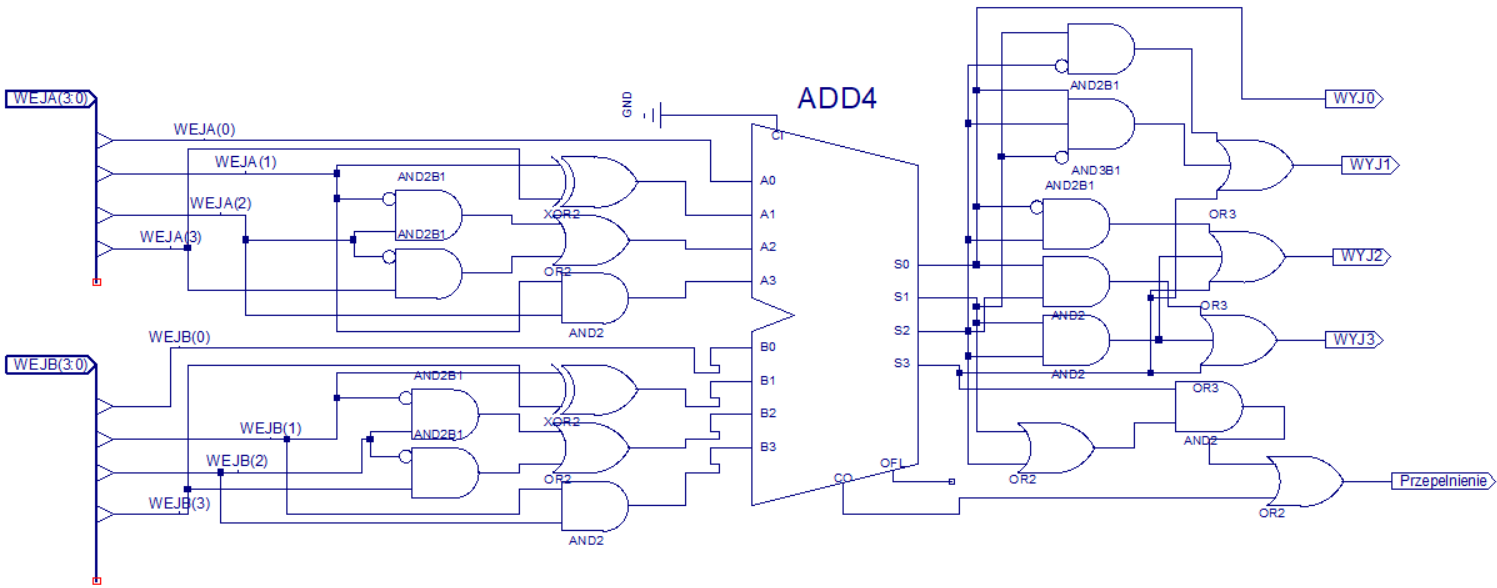
\includegraphics{zadanie2/zad2_scheme.png}
	}
\end{figure}
\subsubsection{Kod VHDL}
\lstinputlisting{zadanie2/testbench.vhd}
\subsubsection{Symulacja}
\begin{figure}[H]
	\centering
	\resizebox*{\textwidth}{!}{
		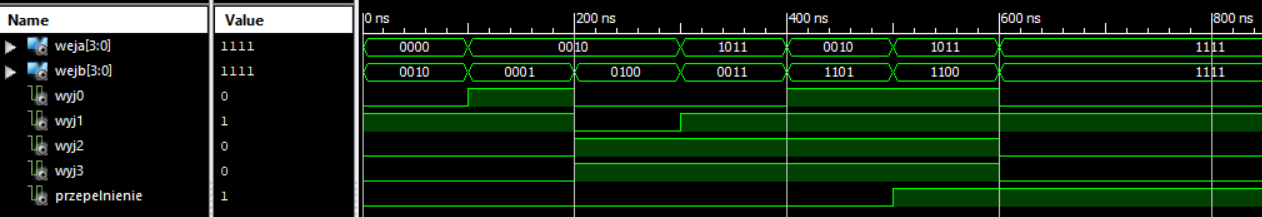
\includegraphics{zadanie2/zad2_simulation.png}
	}
\end{figure}
\subsection{Fizyczna implementacja}
\subsubsection{Kod UCF}
\lstinputlisting{zadanie2/ZL-9572.ucf}
\section{Zadanie 3}
\subsection{Polecenie}
Konwerter cyfry szesnastkowej zapisanej na czterech bitach od 0 do 9, A do F 
na kod ASCII tej cyfry – wyjście 8-bitowe. Prezentacja wyniku na diodach 
przystawki, potem na wyświetlaczu 7-segmentowym. 
\subsection{Rozwiązanie}
\subsubsection{Schemat stanów}
\subsubsection{Tabela prawdy}
\subsubsection{Siatki Karnaugh}
\subsubsection{Schemat układu}
\subsubsection{Kod VHDL}
\subsubsection{Symulacja}
\subsection{Fizyczna implementacja}
\subsubsection{Kod UCF}

\section{Zadanie 4}
\subsection{Polecenie}
Komparator dwóch 4-bitowych cyfr: 2 wejścia po 4 bity, 3 wyjścia 1-bitowe: 
mniejszy, większy, równy pracujący w kodzie Aikena.
\subsection{Rozwiązanie}
\subsubsection{Schemat stanów}
\subsubsection{Tabela prawdy}
\subsubsection{Siatki Karnaugh}
\subsubsection{Schemat układu}
\subsubsection{Kod VHDL}
\subsubsection{Symulacja}
\subsection{Fizyczna implementacja}
\subsubsection{Kod UCF}

\section{Wnioski}
\end{document}